\documentclass{article}
\usepackage[utf8x]{inputenc}
\usepackage{ucs}
\usepackage{amsmath} 
\usepackage{amsfonts}
\usepackage{marvosym}
\usepackage{wasysym}
\usepackage{upgreek}
\usepackage[english,russian]{babel}
\usepackage{graphicx}
\usepackage{float}
\usepackage{textcomp}
\usepackage{hyperref}
\usepackage{geometry}
  \geometry{left=2cm}
  \geometry{right=1.5cm}
  \geometry{top=1cm}
  \geometry{bottom=2cm}
\usepackage{tikz}
\usepackage{ccaption}
\usepackage{multicol}

\hypersetup{
   colorlinks=true,
   citecolor=blue,
   linkcolor=black,
   urlcolor=blue
}

\usepackage{listings}
%\setlength{\columnsep}{1.5cm}
%\setlength{\columnseprule}{0.2pt}

\usepackage[absolute]{textpos}

\usepackage{colortbl,graphicx,tikz}
\definecolor{X}{rgb}{.5,.5,.5}


\begin{document}
\pagenumbering{gobble}
\lstset{
  language=C,                % choose the language of the code
  basicstyle=\linespread{1.1}\ttfamily,
  columns=fixed,
  fontadjust=true,
  basewidth=0.5em,
  keywordstyle=\color{blue}\bfseries,
  commentstyle=\color{gray},
  stringstyle=\ttfamily\color{orange!50!black},
  showstringspaces=false,
  numbersep=5pt,
  numberstyle=\tiny\color{black},
  numberfirstline=true,
  stepnumber=1,                   % the step between two line-numbers.        
  numbersep=10pt,                  % how far the line-numbers are from the code
  backgroundcolor=\color{white},  % choose the background color. You must add \usepackage{color}
  showstringspaces=false,         % underline spaces within strings
  captionpos=b,                   % sets the caption-position to bottom
  breaklines=true,                % sets automatic line breaking
  breakatwhitespace=true,         % sets if automatic breaks should only happen at whitespace
  xleftmargin=.2in,
  extendedchars=\true,
  keepspaces = true,
}
\lstset{literate=%
   *{0}{{{\color{red!20!violet}0}}}1
    {1}{{{\color{red!20!violet}1}}}1
    {2}{{{\color{red!20!violet}2}}}1
    {3}{{{\color{red!20!violet}3}}}1
    {4}{{{\color{red!20!violet}4}}}1
    {5}{{{\color{red!20!violet}5}}}1
    {6}{{{\color{red!20!violet}6}}}1
    {7}{{{\color{red!20!violet}7}}}1
    {8}{{{\color{red!20!violet}8}}}1
    {9}{{{\color{red!20!violet}9}}}1
}
\newpage

\title{Семинар \#10: Сегменты памяти. Классные задания.\vspace{-5ex}}\date{}\maketitle
\section*{Часть 1: Сегменты памяти}
\begin{multicols}{2}
\begin{center}
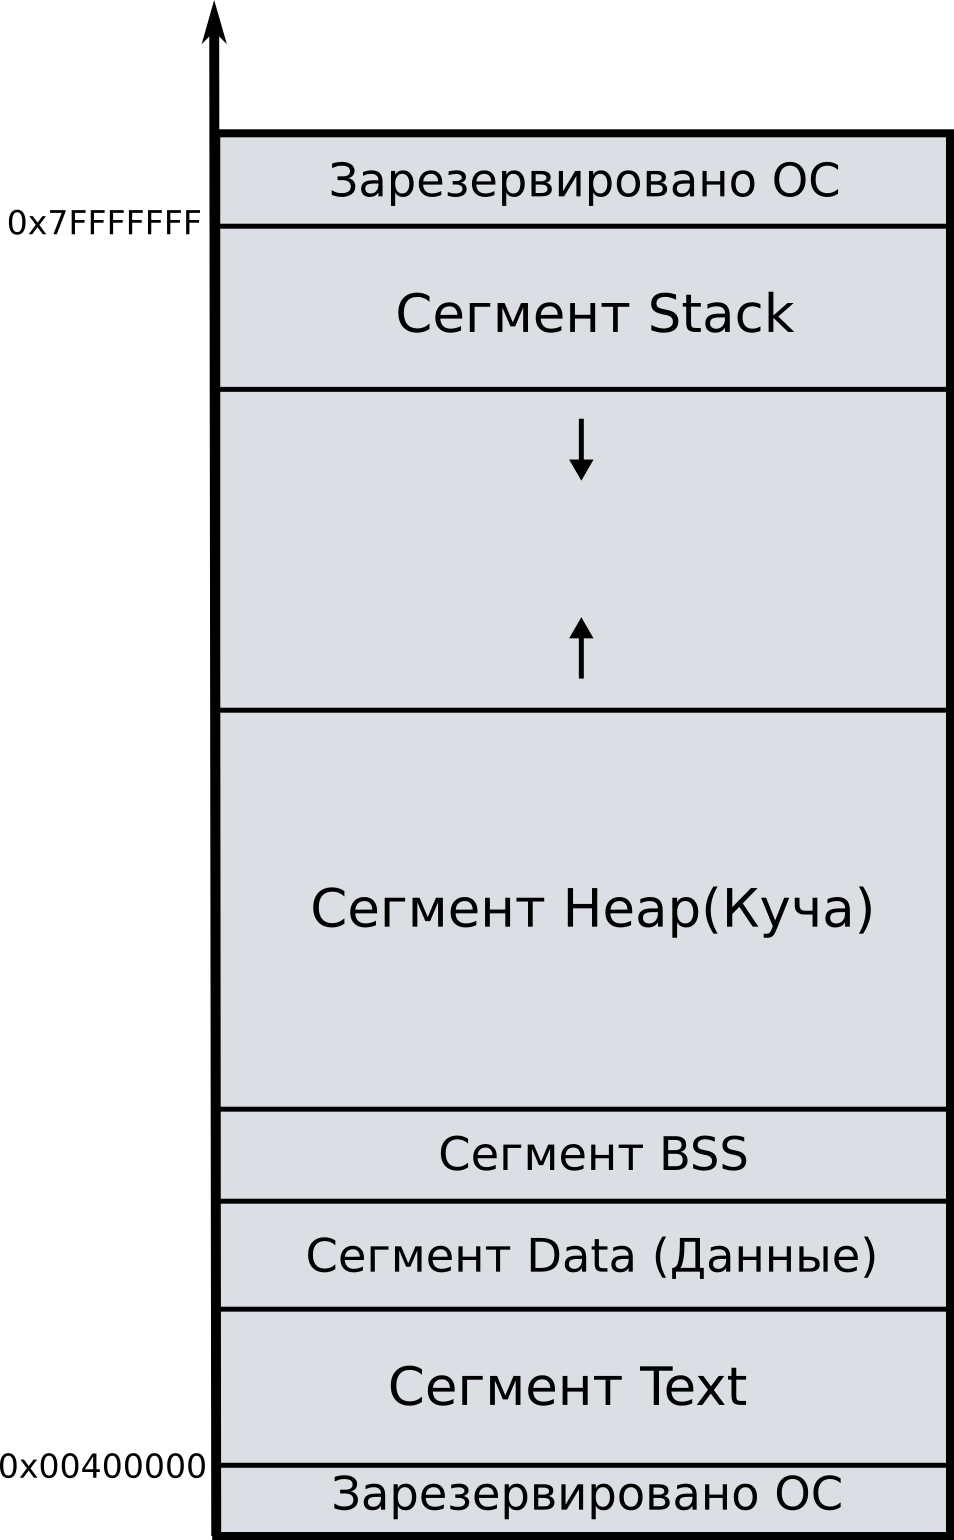
\includegraphics[scale=1.1]{../images/memory_layout.png}
\end{center}
\columnbreak
\begin{enumerate}
\item \textbf{Сегмент памяти Стек (Stack)} \\
\begin{itemize}
\item При обычном объявлении переменных (в том числе массивов) внутри функций все они создаются в стеке: 
\begin{lstlisting}
int a; 
int array[10];
\end{lstlisting}


\item Память на локальные переменные функции выделяется при вызове этой функции и освобождается при завершении функции.
\item Маленький размер (несколько мегабайт, зависит от настроек операционной системы).
\item Выделение памяти происходит быстрее чем в куче
\end{itemize}
\item \textbf{Сегмент памяти Куча (Heap)} \\
\begin{itemize}
\item Выделеть память в куче можно с помощью стандартной функции \texttt{malloc}. \\
\begin{lstlisting}
int* p = malloc(10 * sizeof(int));
\end{lstlisting}
\item Освободить память в куче можно с помощью стандартной функции \texttt{free}
\begin{lstlisting}
free(p);
\end{lstlisting}
\item Память можно выделяется/освобождать в любом месте.
\item Размер ограничен свободной оперативной памятью.
\item Выделение памяти происходит медленней чем в стеке
\end{itemize}
\end{enumerate}
\end{multicols}

\begin{enumerate}
\setcounter{enumi}{2}

\item \textbf{Сегмент памяти Data}
\begin{itemize}
\item В этом сегменте хранятся инициализированные глобальные и статические переменные а также строковые литералы
\end{itemize}

\item \textbf{Сегмент памяти BSS}
\begin{itemize}
\item В этом сегменте хранятся неинициализированные глобальные и статические переменные
\item В большинстве систем все эти данные автоматически инициализируются нулями
\end{itemize}

\item \textbf{Сегмент памяти Text}
\begin{itemize}
\item В этом сегменте хранится машинный код программы (Код на языке C, сначала, переводится в код на языке Ассемблера, а потом в машинный код. Как это происходит смотрите ниже.).
\item Адрес функции - адрес первого байта инструкций в этом сегменте.
\end{itemize}
\end{enumerate}


\subsection*{Создание массива в разных сегментах памяти}
Ниже представлен пример программы в которой создаюся 4 массива в разных сегментах памяти.
\begin{lstlisting}
#include <stdio.h>
#include <stdlib.h>

int array_data[5] = {1, 2, 3, 4, 5};
int array_bss[5];

int main() 
{
    int array_stack[5];
    int* array_heap = (int*)malloc(5 * sizeof(int));
}
\end{lstlisting}
\begin{itemize}
\item Напечатайте адрес начала каждого из массивов. Помните, что для печати адресов используется спецификатор \texttt{\%p}.
\end{itemize}



\subsection*{Переполнение стека -- Stackoverflow}
\begin{itemize}
\item Определите размер стека на вашей системе экспериментальным путём. Создайте массив такого большого размера на стеке, чтобы перестала работать. Минимальный размер массива, при котором падает программа будет примерно равен размеру стека.
\item При каждом вызове функции в стеке хранятся локальные переменные функции, аргументы функции а также адрес возврата функции. Даже функция без локальных переменных и аргументов будет хранить на стеке как минимум адрес возврата (8 байт). Определите размер стека на вашей системе экспериментальным путём с помощью рекурсии.
\end{itemize}

\subsection*{Статические переменные}
Помимо глобальных переменных, в сегменте Data хранятся статические переменные. Такие переменные объявляются внутри функций, но создаются в сегменте Data и не удаляются при завершении функции. Вот пример функции со статической переменной.
\begin{lstlisting}
#include <stdio.h>
void counter() 
{
    static int n = 0;
    n++;
    printf("%i\n", n);
}
int main() 
{
    counter();
    counter();
    counter();
}
\end{lstlisting}
Обратите внмание, что в этой функции строка \texttt{static int n = 0;} не исполняется при заходе в функцию. Эта строка просто объявляет инициализирует статическую переменную, причём инициализация происходит в самом начале исполнения программы (даже до функции \texttt{main}). 

\begin{itemize}
\item Создайте функцию \texttt{adder}, которая будет принимать на вход число и возвращать сумму всех чисел, которые приходили на вход этой функции за время выполнения программы.
\begin{lstlisting}
printf("%i\n", adder(10));  // Напечатает 10
printf("%i\n", adder(15));  // Напечатает 25
printf("%i\n", adder(70));  // Напечатает 95
\end{lstlisting}
\end{itemize}



\newpage
\section*{Часть 2: Динамическое выделение памяти в Куче:}
Основные функции для динамического выделения памяти:
\begin{itemize}
\item \texttt{void* malloc(\textbf{size\_t} n)} -- выделяет \texttt{n} байт в сегменте памяти Куча и возвращает указатель \texttt{void*}
на начало этой памяти. Если память выделить не получилось (например памяти не хватает), то функция вернёт значение \texttt{NULL}. (\texttt{NULL} -- это просто константа равная нулю). \\
\item \texttt{void free(\textbf{void*} p)} -- освобождает выделенную память. Если ненужную память вовремя не освободить, то она останется помеченной, как занятая до момента завершения программы. Произойдёт так называемая утечка памяти.\\
\item \texttt{void* realloc(\textbf{void*} p, \textbf{size\_t} new\_n)} -- перевыделяет выделенную память. Указатель \texttt{p} должен указывать на ранее выделенную память. Память, на которую ранее указывал \texttt{p}, освободится. \\
Если память перевыделить не получилось (например памяти не хватает), то функция вернёт значение \texttt{NULL}. При этом указатель \texttt{p} будет продолжать указывать на старую память, она не освободится.\\
\end{itemize}

Давайте рассмотрим как работать с этими функциями. Предположим, что мы хотим создать на куче одну переменную типа \texttt{int}. Так как мы знаем, что \texttt{int} занимает 4 байта, то мы можем написать следующее.
\begin{lstlisting}
int* p = (int*)malloc(4);
\end{lstlisting}
Обратите внимание на то что мы привели указатель \texttt{void*}, который возвращает \texttt{malloc}, к указателю \texttt{int*}.\\
В языке \texttt{C} такое приведение можно не писать, а в языке \texttt{C++} это обязательно. Однако, такое использование \texttt{malloc} не совсем верно, так как тип \texttt{int} не всегда имеет размер 4 байта. На старых системах он может иметь размер 2 байта, а на очень новых -- даже 8 байт. Поэтому лучше использовать оператор \texttt{sizeof}.\\

Схематически выделение одного \texttt{int}-а в куче можно изобразить следующим образом:
 
\begin{multicols}{2}
\begin{lstlisting}
int* p = (int*)malloc(sizeof(int));
*p = 123;
\end{lstlisting}
\vfill
\columnbreak
\begin{center}
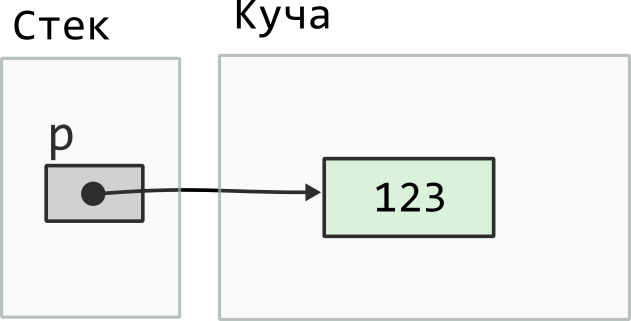
\includegraphics[scale=0.72]{../images/malloc_class_tasks/heap_int.png}
\end{center}
\end{multicols}

Конечно, основное преемущество кучи это её размер, который ограничен только доступной физической памятью. Поэтому на куче обычно выделяют не одиночные переменные, а массивы. Вот схематическое изображение выделения массива из 4-х элементов на куче:
\begin{multicols}{2}
\begin{lstlisting}
int* p = (int*)malloc(4 * sizeof(int));
p[0] = 11;
p[1] = 22;
p[2] = 33;
p[3] = 44;
\end{lstlisting}
\vfill
\columnbreak
\begin{center}
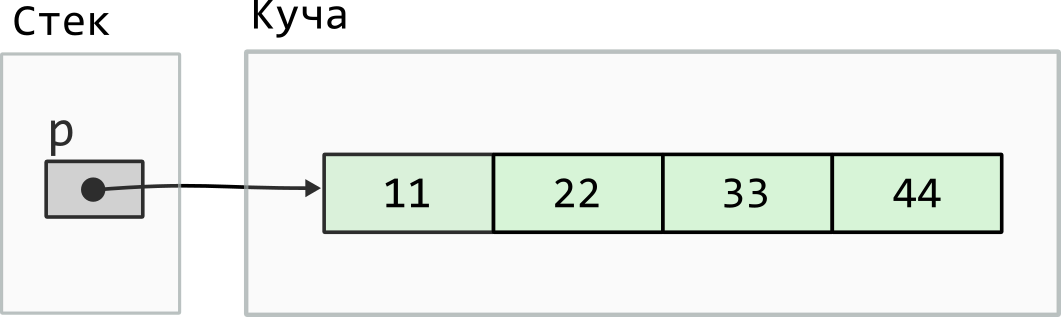
\includegraphics[scale=0.72]{../images/malloc_class_tasks/heap_int_array.png}
\end{center}
\end{multicols}
Благодаря тому, что к указателям можно применять квадратные скобки, работа с указателем \texttt{p} ничем не отличается от работы с массивом размером в 4 элемента.\\
После того как вы поработали с памятью в куче и она стала вам не нужна, память нужно освободить так:
\begin{lstlisting}
free(p);
\end{lstlisting}
Если это не сделать, то выделенные в куче объекты будут занимать память даже когда они уже перестали быть нужны. Эта память освободится только при завершении программы. Правило при работе с \texttt{free}: число вызовов \texttt{free} должно быть равно числу вызовов \texttt{malloc}.



\newpage
\subsubsection*{Задачи:}

Напишите код, который будет создавать в куче объекты, соответствующие следующим рисункам. В каждой задаче напечатайте созданные в куче объекты. В каждой задаче освободите всю память, которую вы выделили.
\begin{itemize}
\item Один символ.
\begin{center}
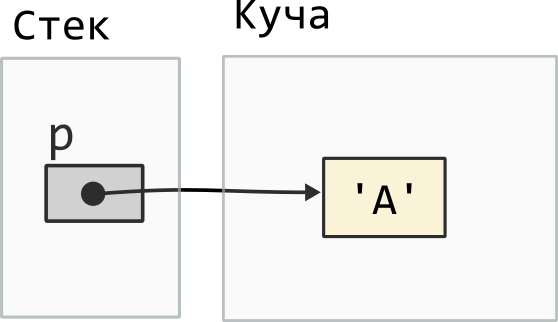
\includegraphics[scale=0.72]{../images/malloc_class_tasks/heap_char.png}
\end{center}


\item Массив из трёх элементов типа \texttt{double}.
\begin{center}
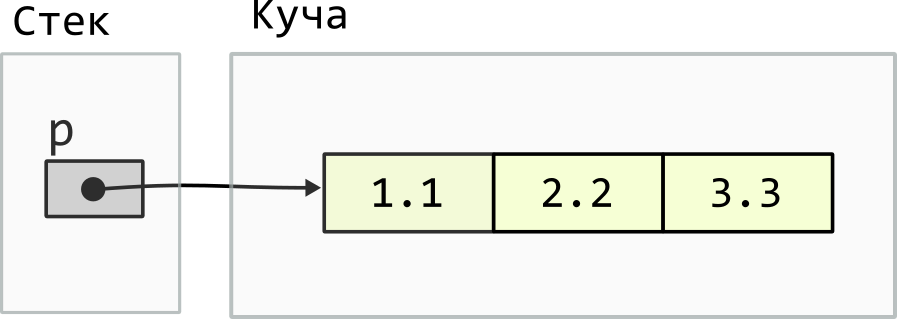
\includegraphics[scale=0.72]{../images/malloc_class_tasks/heap_double_array.png}
\end{center}

\item Строку (массив \texttt{char}) \texttt{"Cats and Dogs"}. Чему должен быть равен размер массива символов? Для присваивания значения строке используйте функцию \texttt{strcpy}.
\begin{center}
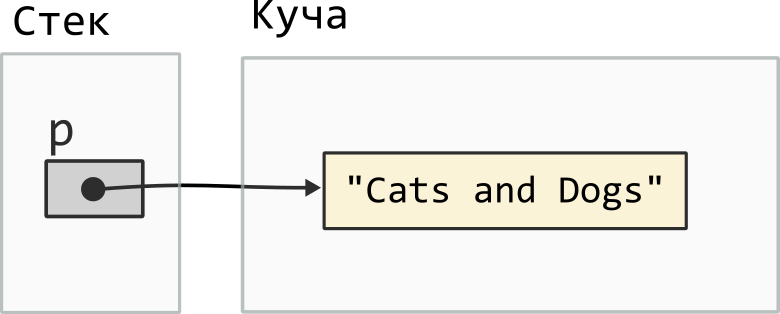
\includegraphics[scale=0.72]{../images/malloc_class_tasks/heap_char_array.png}
\end{center}


\item Структуру \texttt{Book} из семинара на структуры. Для присваивания значения строке используйте \texttt{strcpy}.
\begin{center}
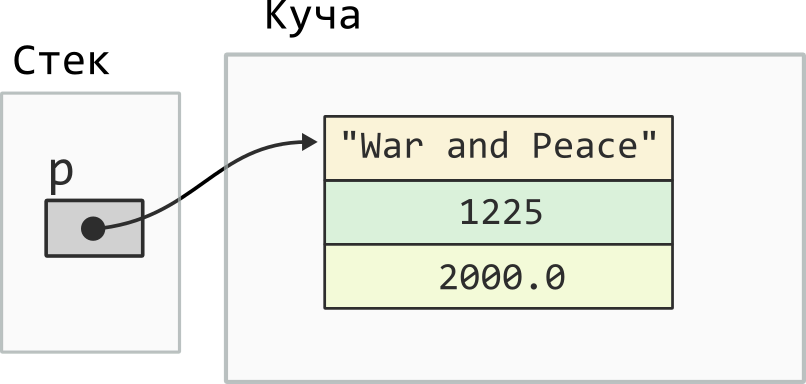
\includegraphics[scale=0.72]{../images/malloc_class_tasks/heap_struct_book.png}
\end{center}


\item Указатель, который указывает на число \texttt{int}.
\begin{center}
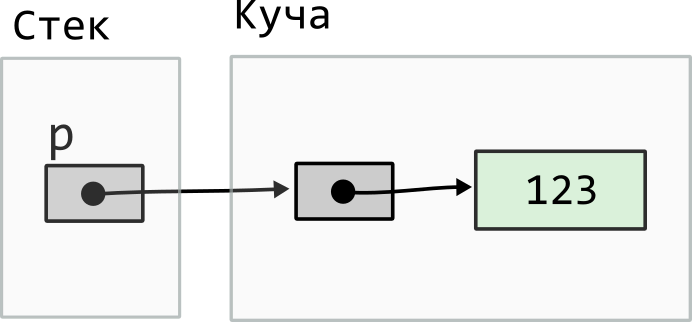
\includegraphics[scale=0.72]{../images/malloc_class_tasks/heap_pointer_int.png}
\end{center}
В этом случае нужно использовать 2 вызова \texttt{malloc} и 2 вызова \texttt{free}.

\newpage
\item Указатель, который указывает на число \texttt{int}, которое находится в стеке.
\begin{center}
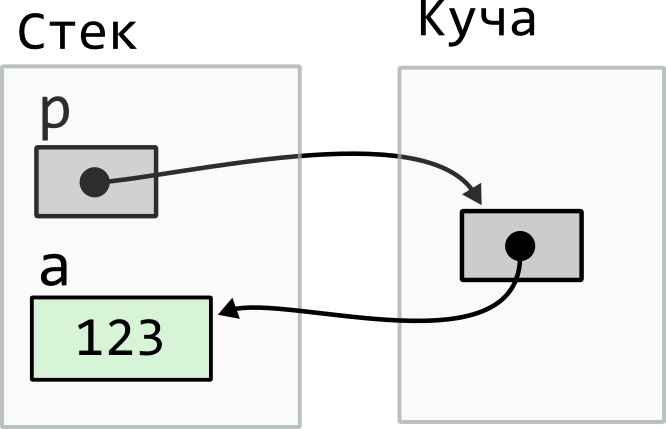
\includegraphics[scale=0.72]{../images/malloc_class_tasks/heap_pointer_int_stack.png}
\end{center}

\item Массив из указателей на \texttt{int}.
\begin{center}
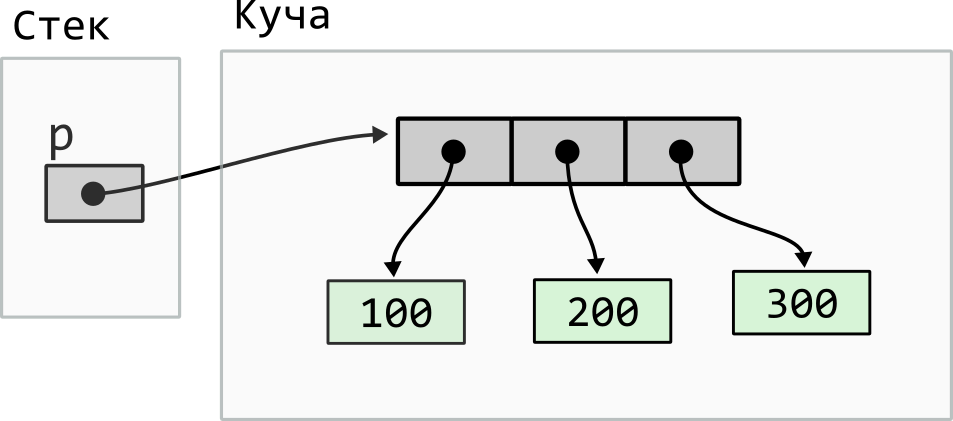
\includegraphics[scale=0.83]{../images/malloc_class_tasks/heap_pointer_array.png}
\end{center}
В этой задаче нужно использовать 4 вызова \texttt{malloc} и 4 вызова \texttt{free}.

\item Пусть есть структура, которая хранит 2 указателя: \texttt{numbers} и \texttt{symbols}:
\begin{lstlisting}
struct data 
{
    int* numbers;
    char* symbols;
};
typedef struct data Data;
\end{lstlisting}

Используйте эту структуру, чтобы выделить память в куче следующим образом:
\begin{center}
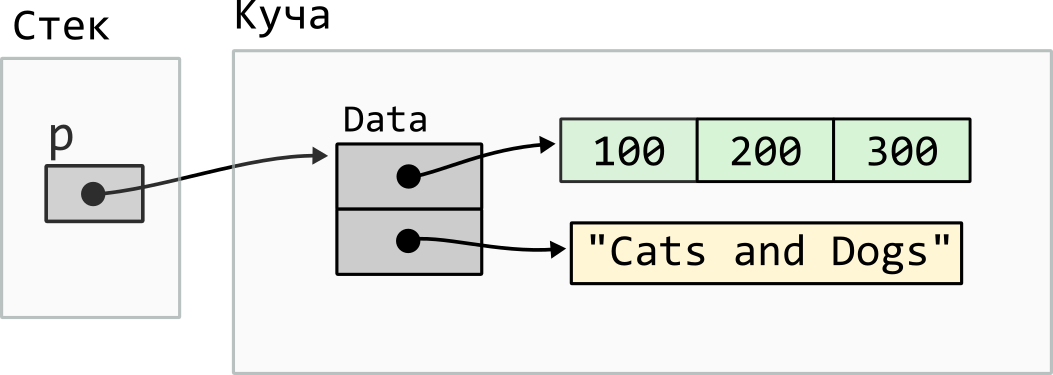
\includegraphics[scale=0.83]{../images/malloc_class_tasks/heap_struct_with_pointers.png}
\end{center}
В этой задаче нужно использовать 3 вызова \texttt{malloc} и 3 вызова \texttt{free}.
\end{itemize}


\newpage
\section*{Часть 3: Ошибки при использовании динамического выделения памяти}

\subsection*{Утечки памяти}
Если вы забудете освободить память с помощью \texttt{free}, когда она перестанет быть нужна, то программа будет использовать больше памяти чем нужно. Произойдёт так называемая утечка памяти. Если в программе есть утечки памяти, то с течением времени она будет потреблять всё больше и больше памяти. При завершении программы всё память, конечно, освобождается.
\begin{lstlisting}
#include <stdlib.h>
void func(int n) 
{
    int* p = (int*)malloc(n * sizeof(int));
    // ...
}

int main() 
{
    func(10000);
    // После выполнения функции func мы не сможем освободить память, даже если захотим
    // так как не знаем указатель на начало этой памяти
    
    // При каждом вызове функции будет тратиться память
    for (int i = 0; i < 100; ++i)
        func(10000);
}
\end{lstlisting}
Существуют специальные программы, которые проверяют нет ли у вас в программе утечек памяти. Одна из таких программ -- \texttt{valgrind} на ОС семейства \texttt{Linux}. Чтобы её использовать, нужно просто написать в терминале:
\begin{verbatim}
valgrind ./a.out
\end{verbatim}

\begin{itemize}
\item Протестируйте программу в файле \texttt{code/memory\_leak.cpp} с помощью \texttt{valgrind}.
\item Исправьте утечку памяти в той программе и снова протестируйте её с помощью \texttt{valgrind}.
\end{itemize}

\subsection*{Ошибка при выделении памяти}
Если при вызове \texttt{malloc} произошла какая-либо ошибка, например, вы просите больше памяти, чем осталось, то \texttt{malloc} вернёт нулевой указатель равный \texttt{NULL} (то есть \texttt{0}). Поэтому при каждом вызове \texttt{malloc} желательно проверять, сработал ли он корректно:
\begin{lstlisting}
int* p = (int*)malloc(1000 * sizeof(int));
if (p == NULL) 
{
    printf("Error! Out of memory.\n");
    exit(1);
}
\end{lstlisting}

\subsection*{Повторное освобождение той же памяти}
Если вы попробуете освободить уже освобождёнынй участок памяти
\begin{lstlisting}
int* p = (int*)malloc(1000 * sizeof(int));
free(p);
free(p);
\end{lstlisting}

\end{document}